\documentclass[landscape,a2paper,fontscale=0.62]{baposter}

\usepackage{multicol} % This is so we can have multiple columns of text side-by-side
\columnsep=100pt % This is the amount of white space between the columns in the poster
\columnseprule=3pt % This is the thickness of the black line between the columns in the poster

%\usepackage{times} % Use the times font
%\usepackage{palatino} % Uncomment to use the Palatino font
\usepackage{kpfonts, baskervald}

\usepackage{graphicx} % Required for including images
\usepackage{booktabs} % Top and bottom rules for table
\usepackage[font=small,labelfont=bf]{caption} % Required for specifying captions to tables and figures
\usepackage{amsfonts, amsmath, amsthm, amssymb} % For math fonts, symbols and environments
\usepackage{wrapfig} % Allows wrapping text around tables and figures
\usepackage{graphicx,caption,float}
\usepackage{bbm}
\usepackage{bbold}
\usepackage{amsthm}
\usepackage{amsmath}
\usepackage{xcolor}
\usepackage{url,hyperref}
\usepackage{amssymb}
\usepackage{amsfonts}
\usepackage{listings}
\usepackage{mwe}
\usepackage[toc,page]{appendix}
\usepackage{enumitem}
\usepackage[noend]{algpseudocode}
\usepackage[english]{babel}
\usepackage[utf8]{inputenc}
\usepackage{listings}
\newtheorem{theorem}{Theorem}
\usepackage{color}
\usepackage{subfig}
\usepackage{multirow}
\usepackage{array}
\usepackage{mathtools}

\usepackage{pifont}
\renewcommand{\labelitemi}{\ding{229}}
\renewcommand{\labelitemii}{\ding{228}}
\renewcommand{\labelitemiii}{\ding{225}}

\setlength\floatsep{1\baselineskip plus 3pt minus 2pt}
\setlength\textfloatsep{1\baselineskip plus 3pt minus 2pt}
\setlength\intextsep{0pt}

\graphicspath{{images/}}
\usepackage{etoolbox}
\patchcmd{\thebibliography}{\section*{\refname}}{}{}{}

\begin{document}
%% Format it to your taste with the options
\background{
      \begin{tikzpicture}[remember picture,overlay]%
      \draw (current page.north west)+(-2em,2em) node[anchor=north west]
      {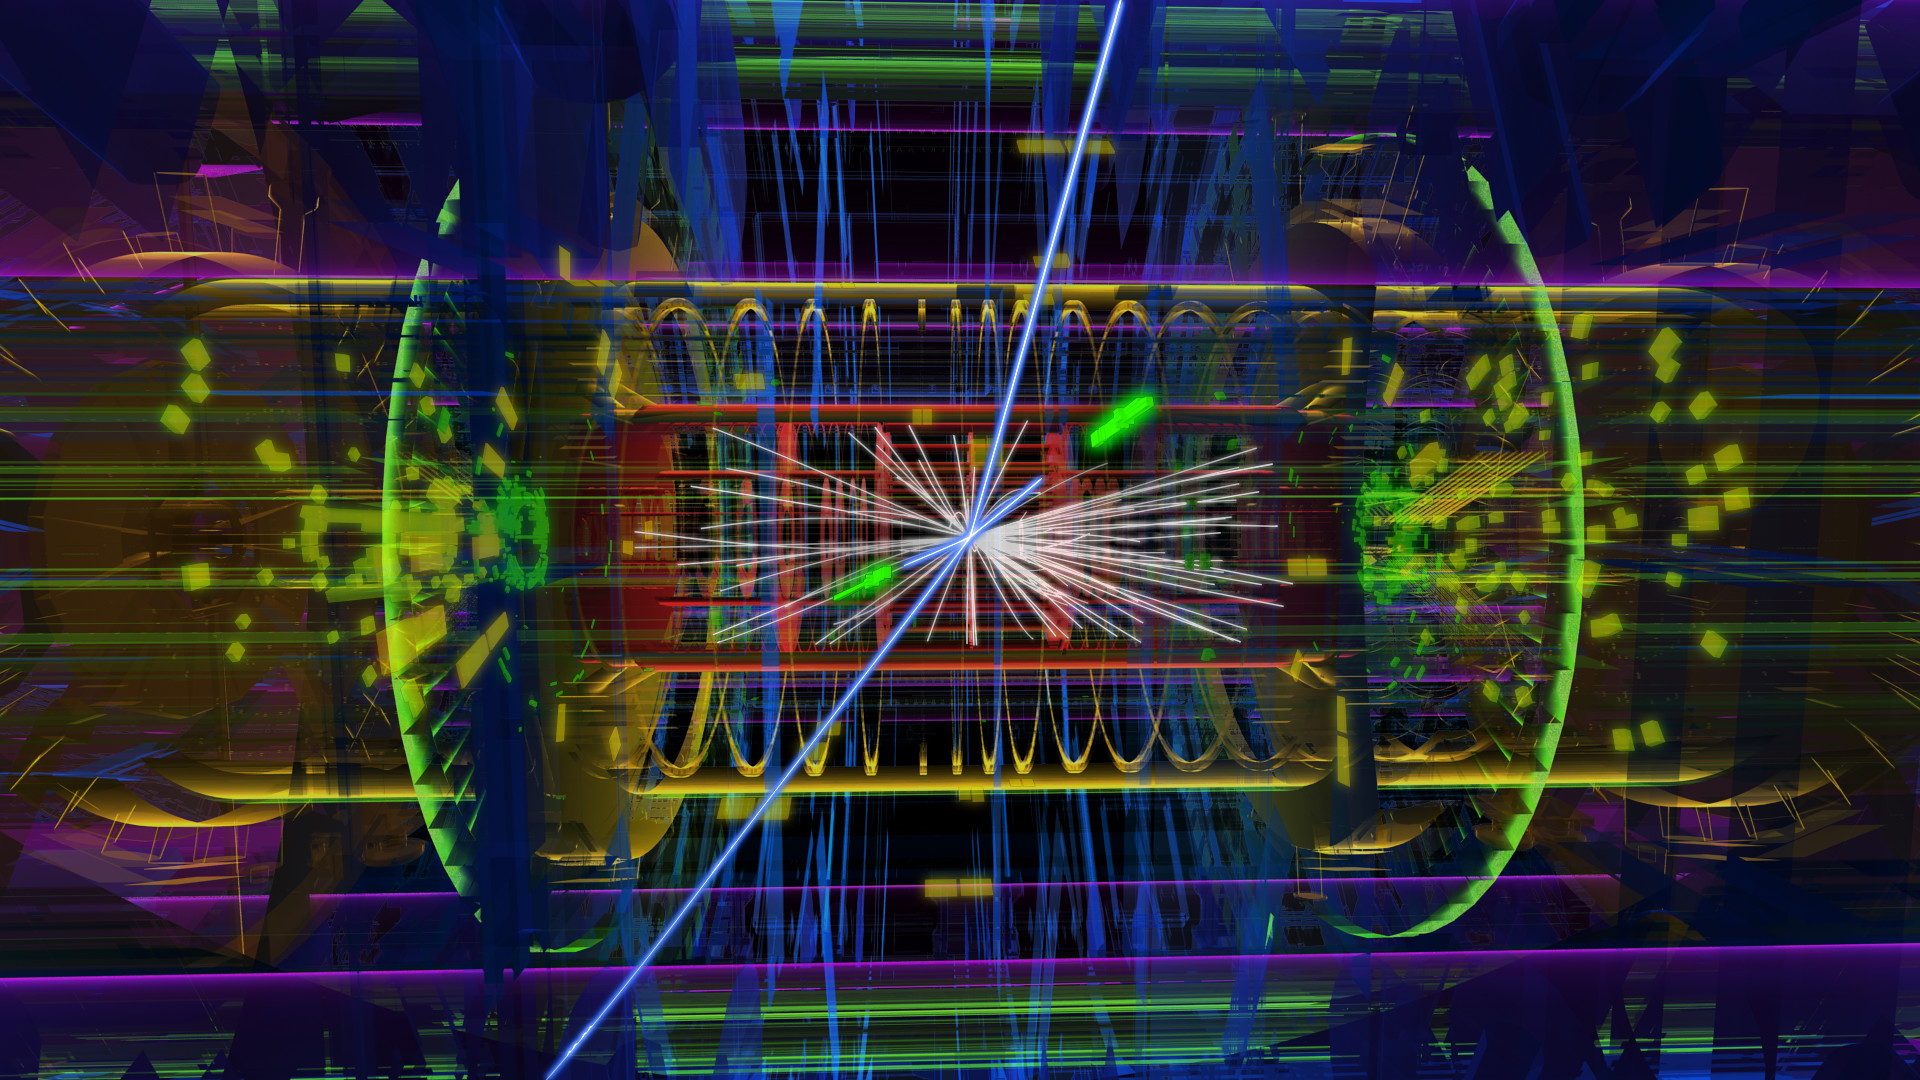
\includegraphics[height=1.2\textheight]{cern}};
      \end{tikzpicture}%
      }
\begin{poster}{
 % Show grid to help with alignment
 grid=false,
 % Column spacing
 colspacing=0.7em,
 % Color style
 headerColorOne=violet!90!white!50,
 borderColor=violet!90!white!50,
 % Format of textbox
 textborder=roundedsmall,
 % Format of text header
 headerborder=closed,
 headershape=roundedright,
 headershade=plain,
 background=user,
 %bgColorOne=white!100,
 boxshade = plain,
 headerheight=0.12\textheight
}
{
  \begin{tabular}{r}
    
\includegraphics[height=0.1\textheight]{inv}
  \end{tabular}
}
 % Title
 {\color{white} \sc{\Huge Numerical Solutions to Quarkonia Wavefunctions}}
 % Authors
 {\color{white}
 {Matthew Rossetter}\\
 {Physics Problem Solving Computing Project}\\
 {Supervisor: Dr Ben Pecjak}\\
}
 % University logo
{
  \begin{tabular}{r}
    
\includegraphics[height=0.1\textheight]{logo0}
  \end{tabular}
 }

\headerbox{Introduction}{name=intro,column=0,row=0,span=2,boxColorOne=white}{
    Quarks are fundamental particles of the Standard Model of particle physics, most well-known for being the constituent particles of the proton and neutron. 
    They \textbf{cannot exist as free particles,} and so will only exist inside of composite particles with other quarks, such as the proton. 
    They can form quark-antiquark pairs known as mesons - these particles can be studied similarly to the Hydrogen atom. 
  }

%\headerbox{Motivation}{name=moti,below=intro,column=0,span=1,boxColorOne=white}{
%    Is this really necessary?
%}
\headerbox{Theory}{name=theory,below=intro,above=bottom,column=0, span=1,boxColorOne=white}{
    \begin{align}
        -\frac{\hbar^2}{2\mu}\nabla^2\psi &+ [V(r) - E_{nl}]\psi = 0 \\
        V(r) &= -\frac{4\alpha_s}{3r} + \beta r
    \end{align}
    Radial wavefunction, $u_{nl}(r) = rR_{nl}(r)$
    \begin{align}
        \frac{du_{nl}}{dr} &= v_{nl} \\
        \frac{dv_{nl}}{dr} &= \frac{l(l+1)}{r^2}u_{nl} - 2\mu[E_{nl}-V(r)]u_{nl}
    \end{align}
  }


\headerbox{The Bisection Method}{name=bis,below=intro,column=1,span=1,boxColorOne=white}{
    The correct $u_{nl}$ can be found using the \textbf{bisection method.}
    This method guess three energies, $E_1, E_3$, and $E_2 = \frac{E_1+E_3}{2}$.
    Equations (3) and (4) can be solved for these energies using \texttt{scipy.integrate.odeint} or a similar ode solver. 
    Count the nodes and turning points for each function - if these differ between two solutions, $E_{nl}$ lies somewhere between those energies. 
    \begin{figure}[H]
        \centering
        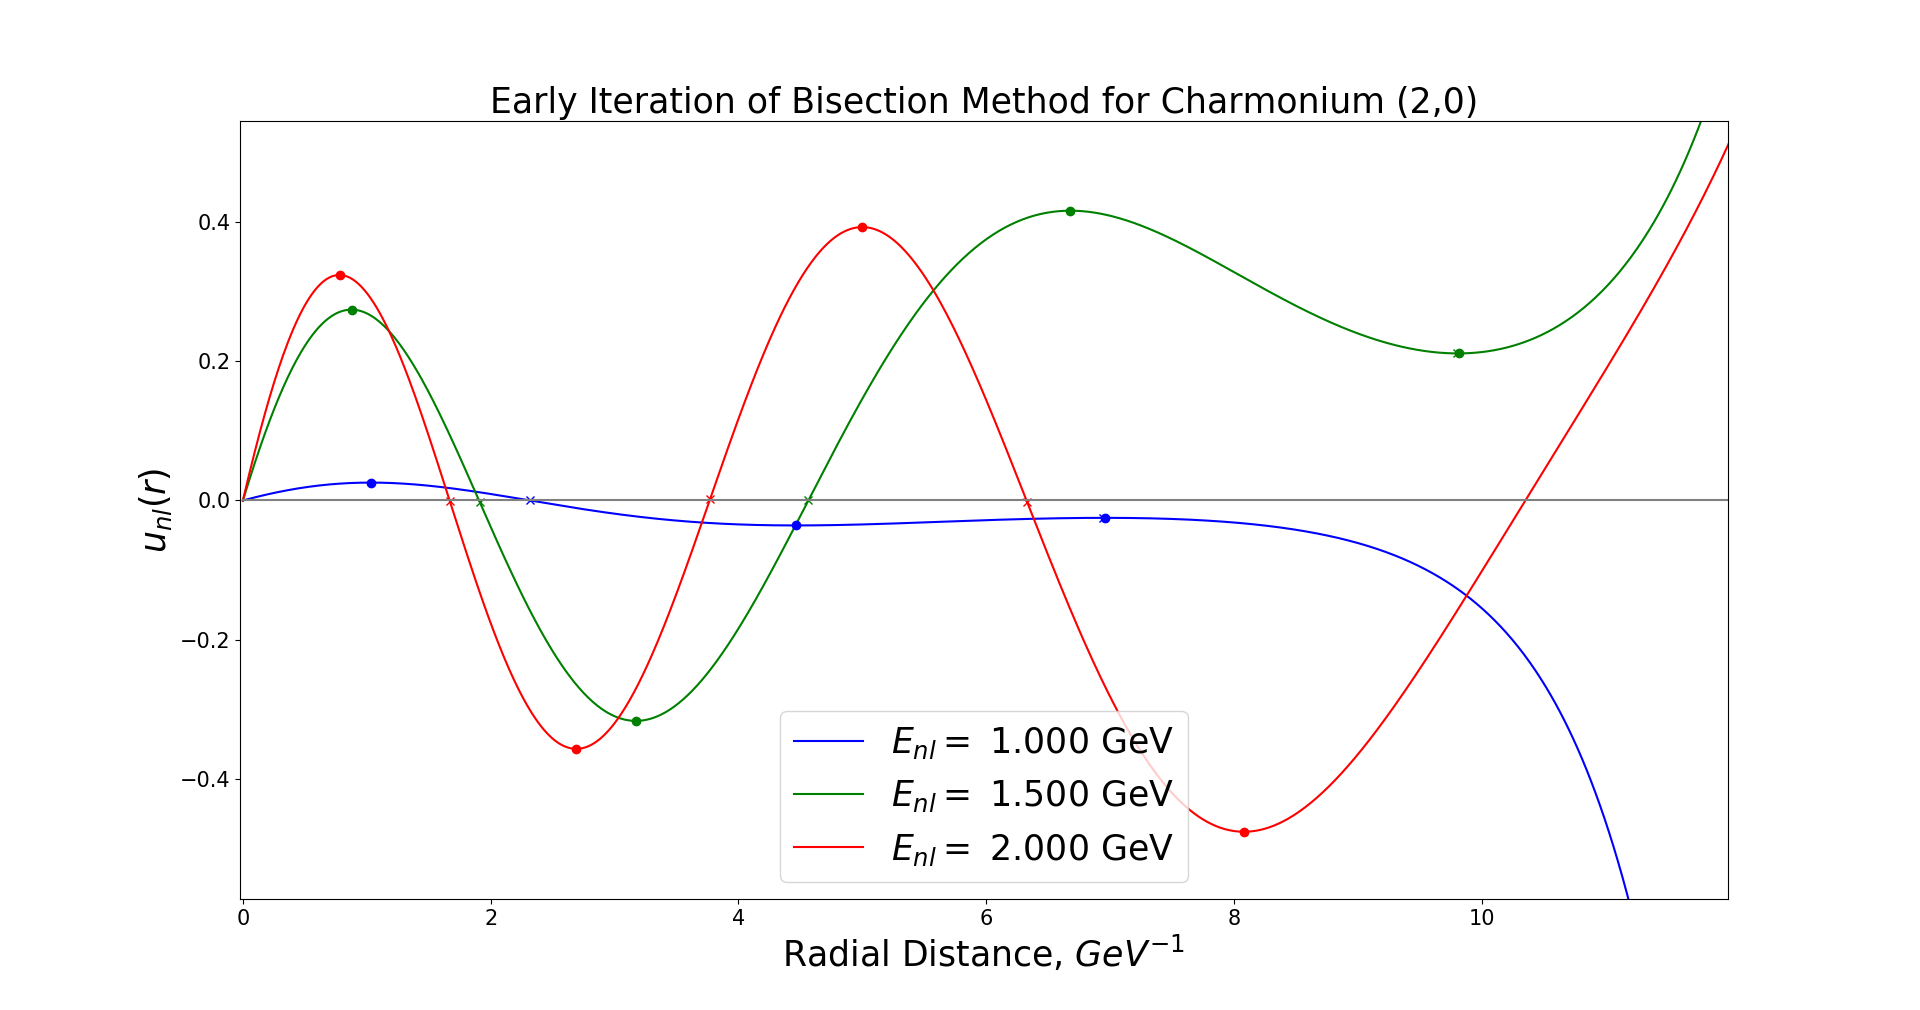
\includegraphics[width=\linewidth]{nodes}
    \end{figure}
    $E_1$ and $E_3$ are set to the two energies over the difference, and $E_2$ calculated again. 
    A correct solution to $u_{nl}$ will have $(n-1)$ nodes and $n$ turning points, as energies converge on $E_{nl}$.
}

\headerbox{References}{name=references,column=2,span=2,above=bottom,boxColorOne=white}{
\nocite{*} % Print all references regardless of whether they were cited in the poster or not
\bibliographystyle{plain} % Plain referencing style
\bibliography{sample} % Use the example bibliography file sample.bib
   }

\headerbox{Results of Computations}{name=comp,above=references,column=2,span=1,boxColorOne=white}{
%    \begin{figure}[H]
%        \centering
%        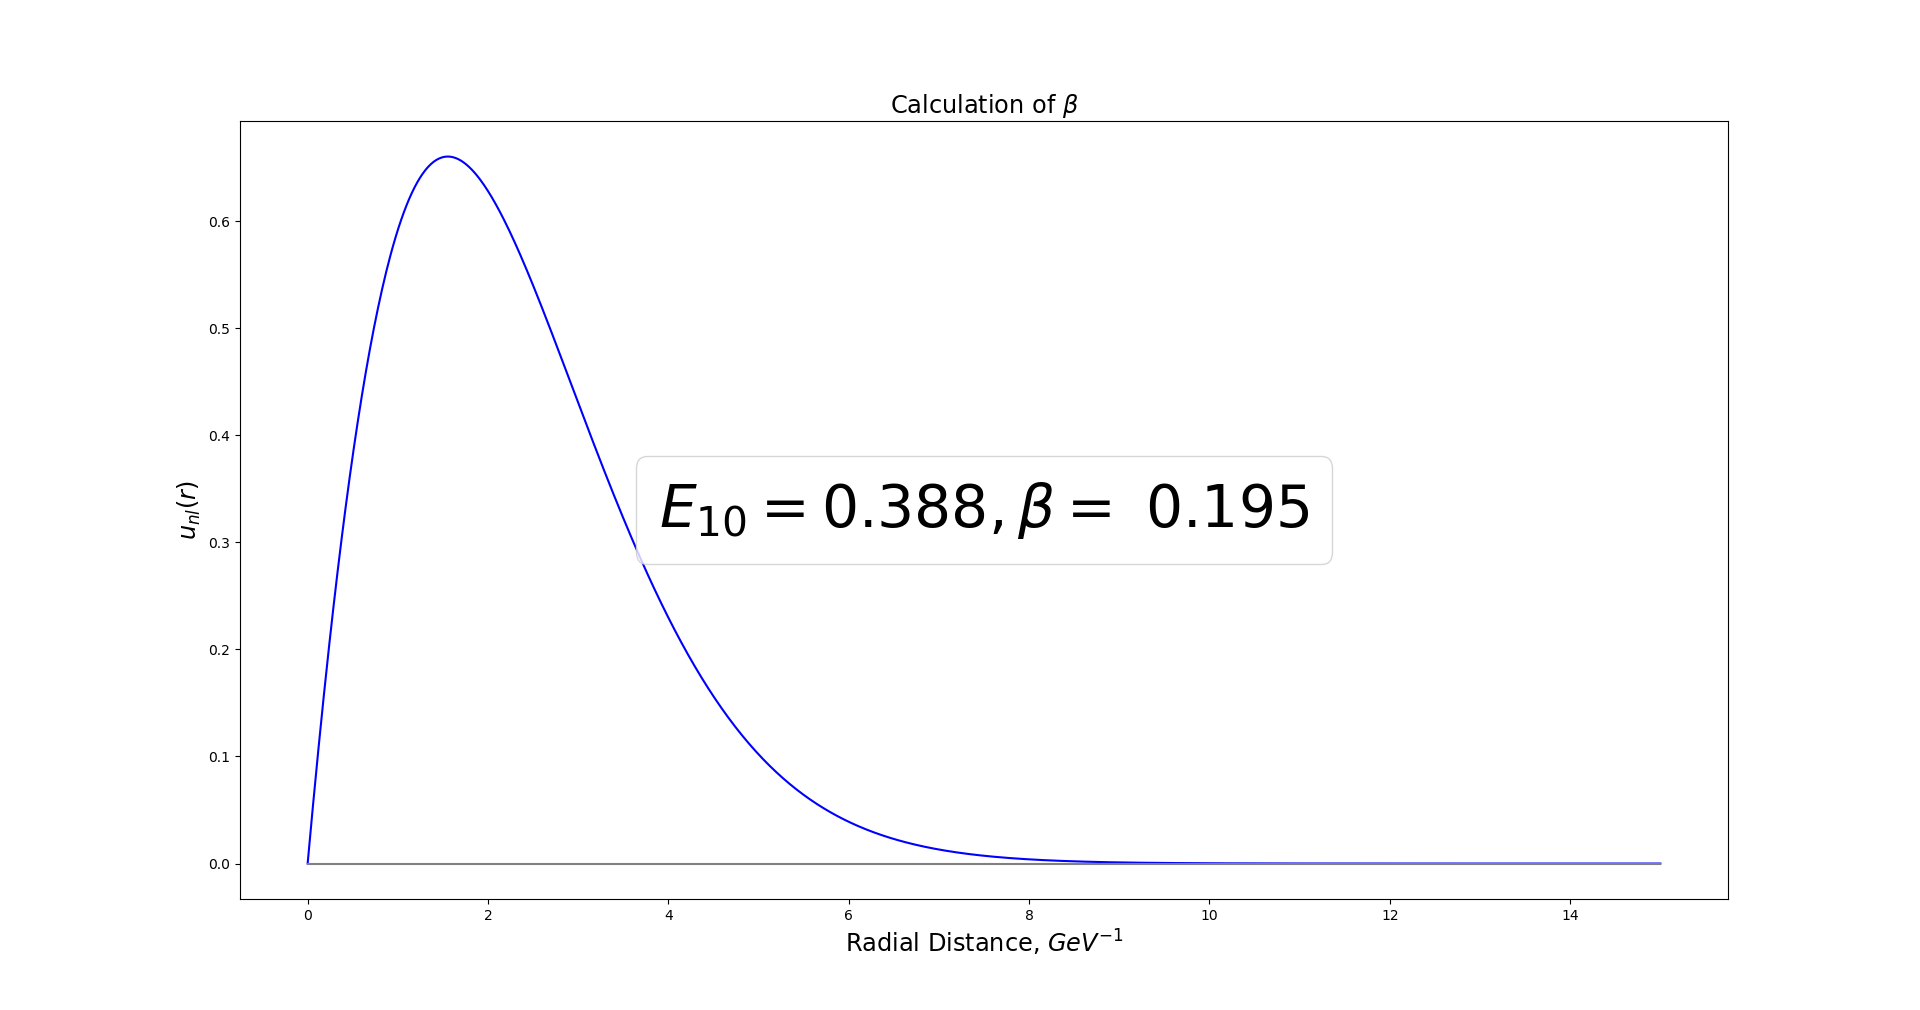
\includegraphics[width=\linewidth]{beta}
%    \end{figure}
    \begin{figure}[H]
        \centering
        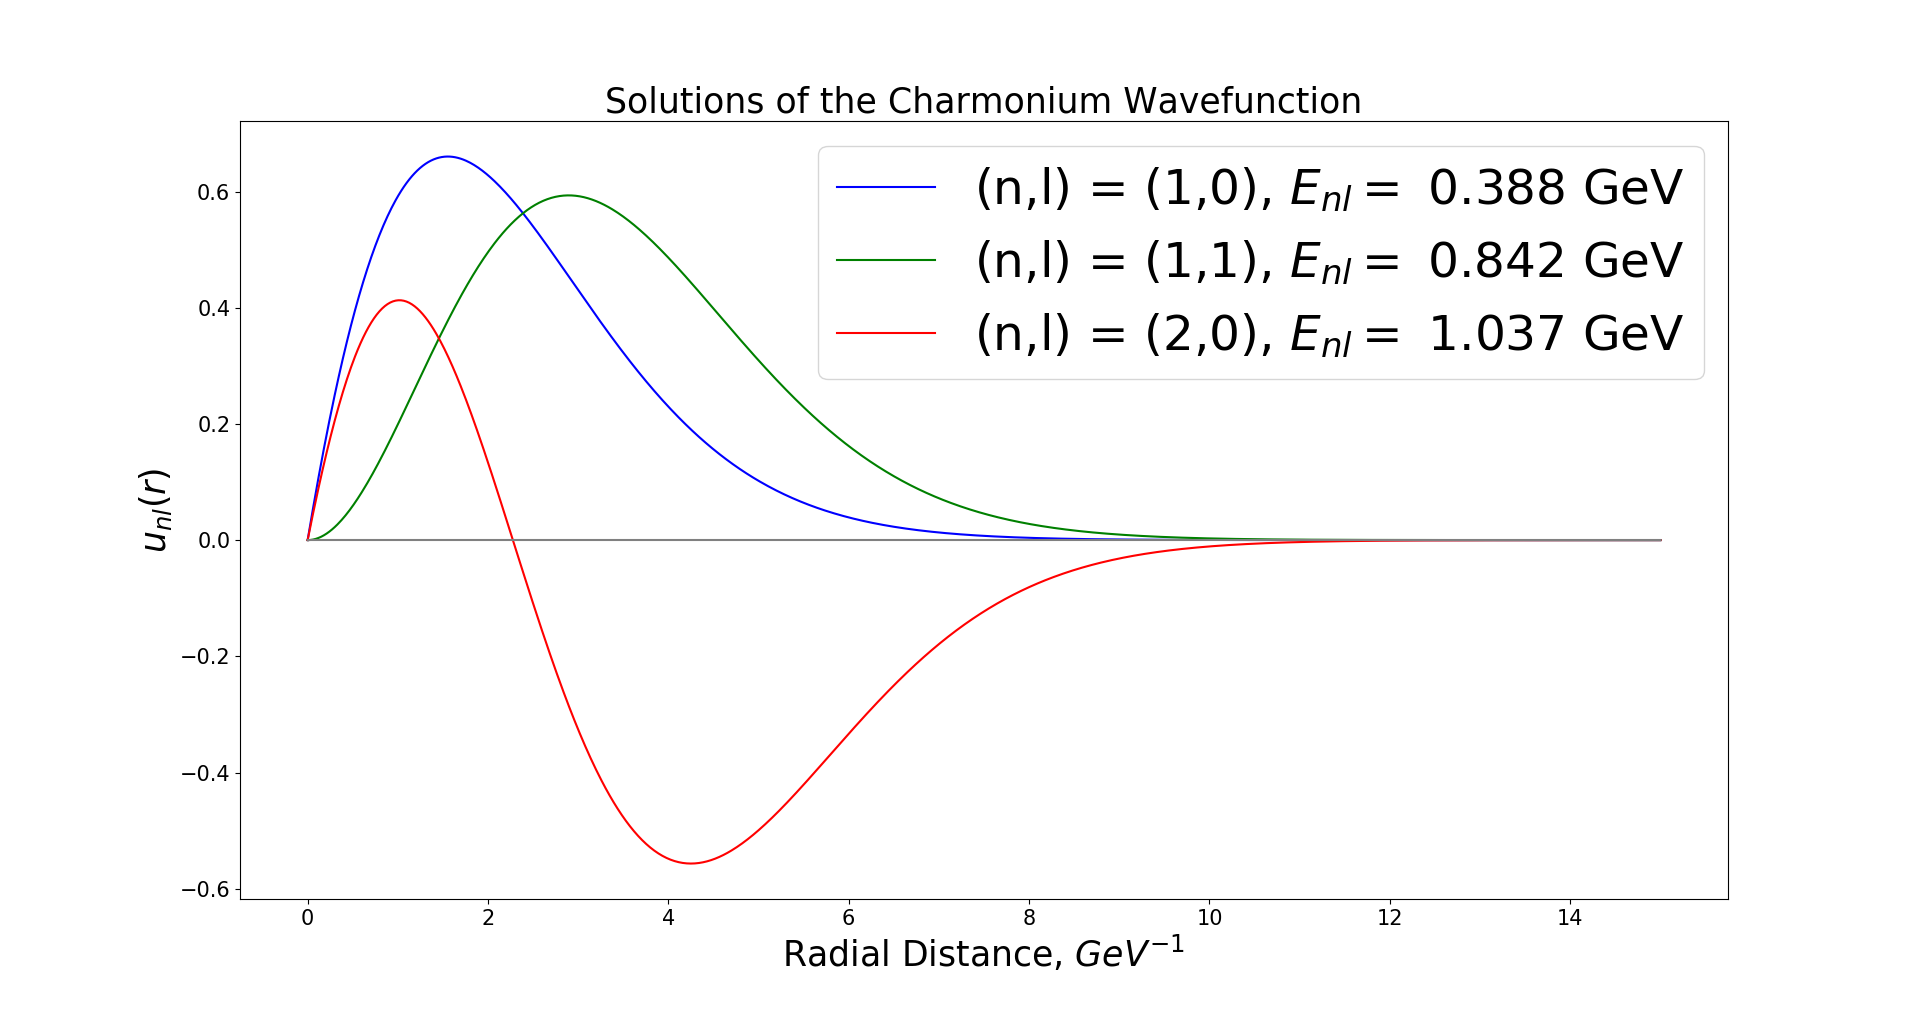
\includegraphics[width=\linewidth]{Charmonium}
    \end{figure}
}

\headerbox{Outlook}{name=outlook,column=3,span=1,boxColorOne=white}{
}

\headerbox{Faults of the Method}{name=faults,column=3, above=references, below=outlook, boxColorOne=white}{
    \begin{figure}[H]
        \centering
        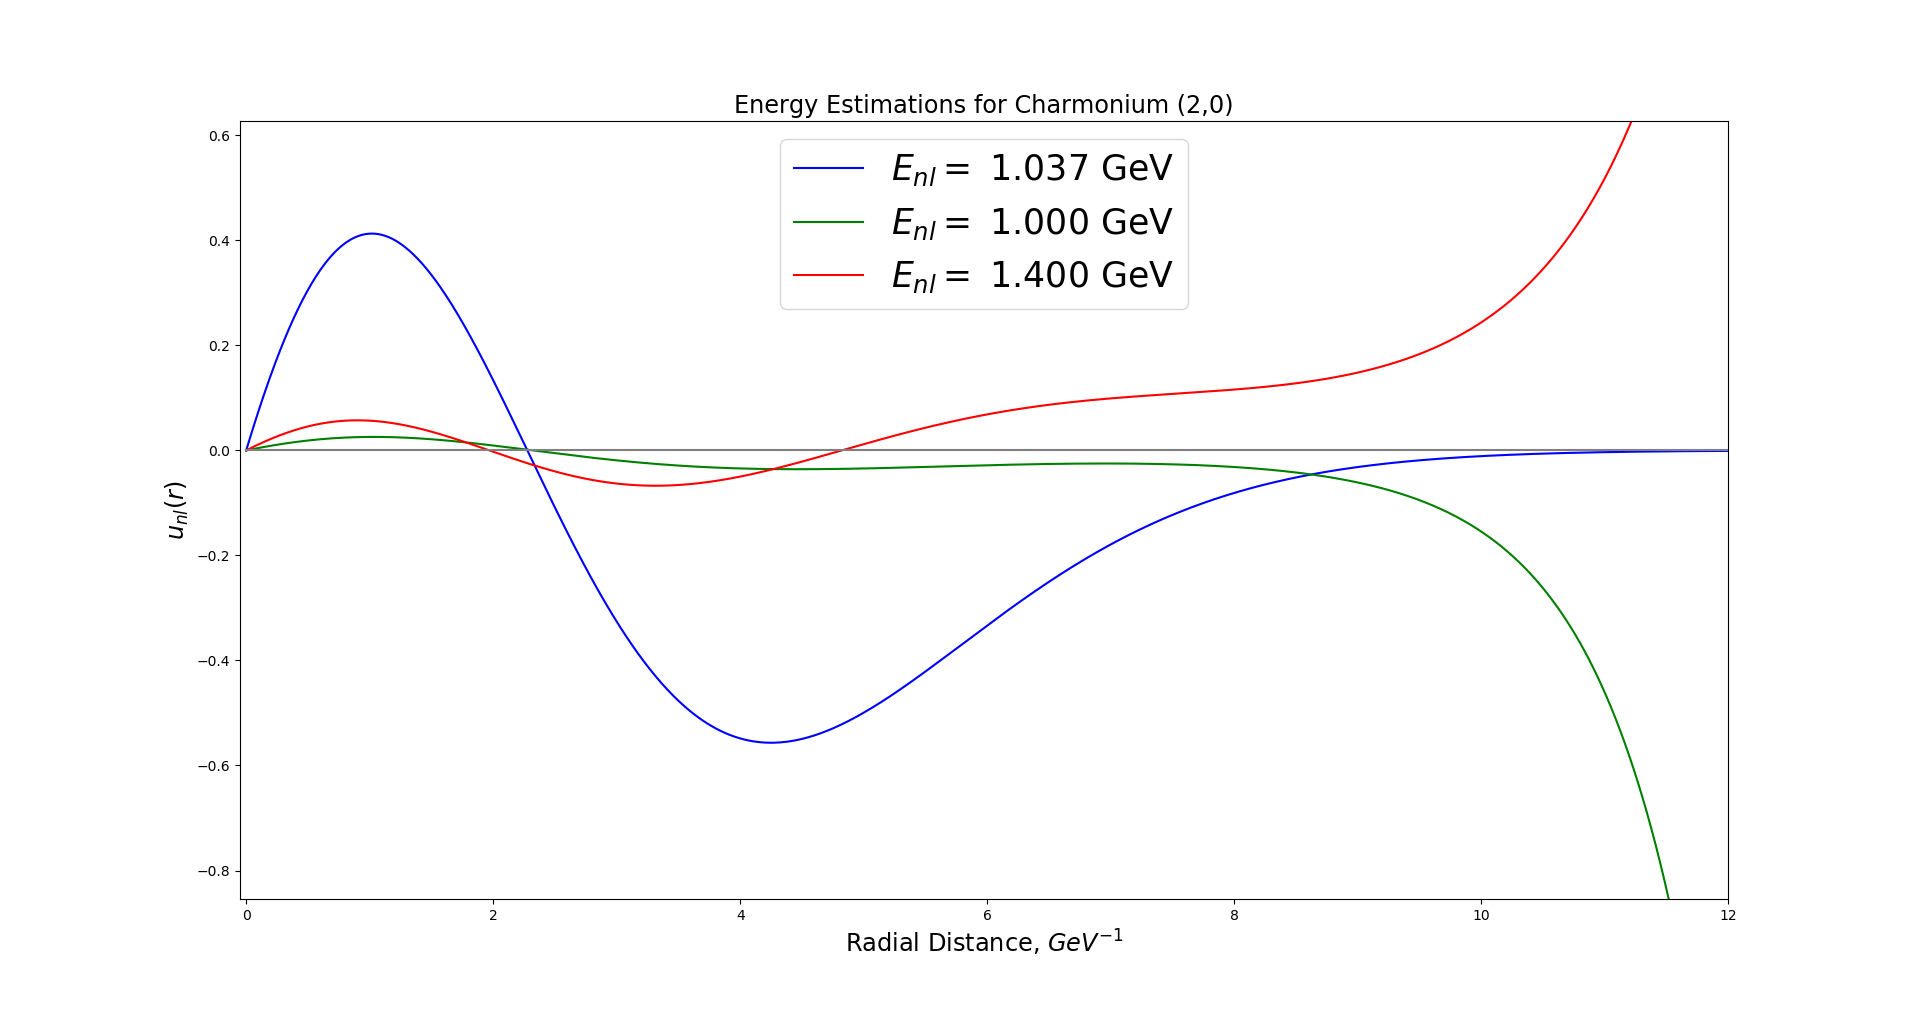
\includegraphics[width=\linewidth]{div}
    \end{figure}
   }




\headerbox{The Hydrogen Wavefunction}{name=hydro,column=1,below=bis,above=bottom,span=1,boxColorOne=white}{
    \begin{equation}
        \frac{4\alpha_s}{3} \to \alpha = \frac{1}{137},~ \beta \to 0,~ \mu \to m_e
    \end{equation}
    \begin{figure}[H]
        \centering
        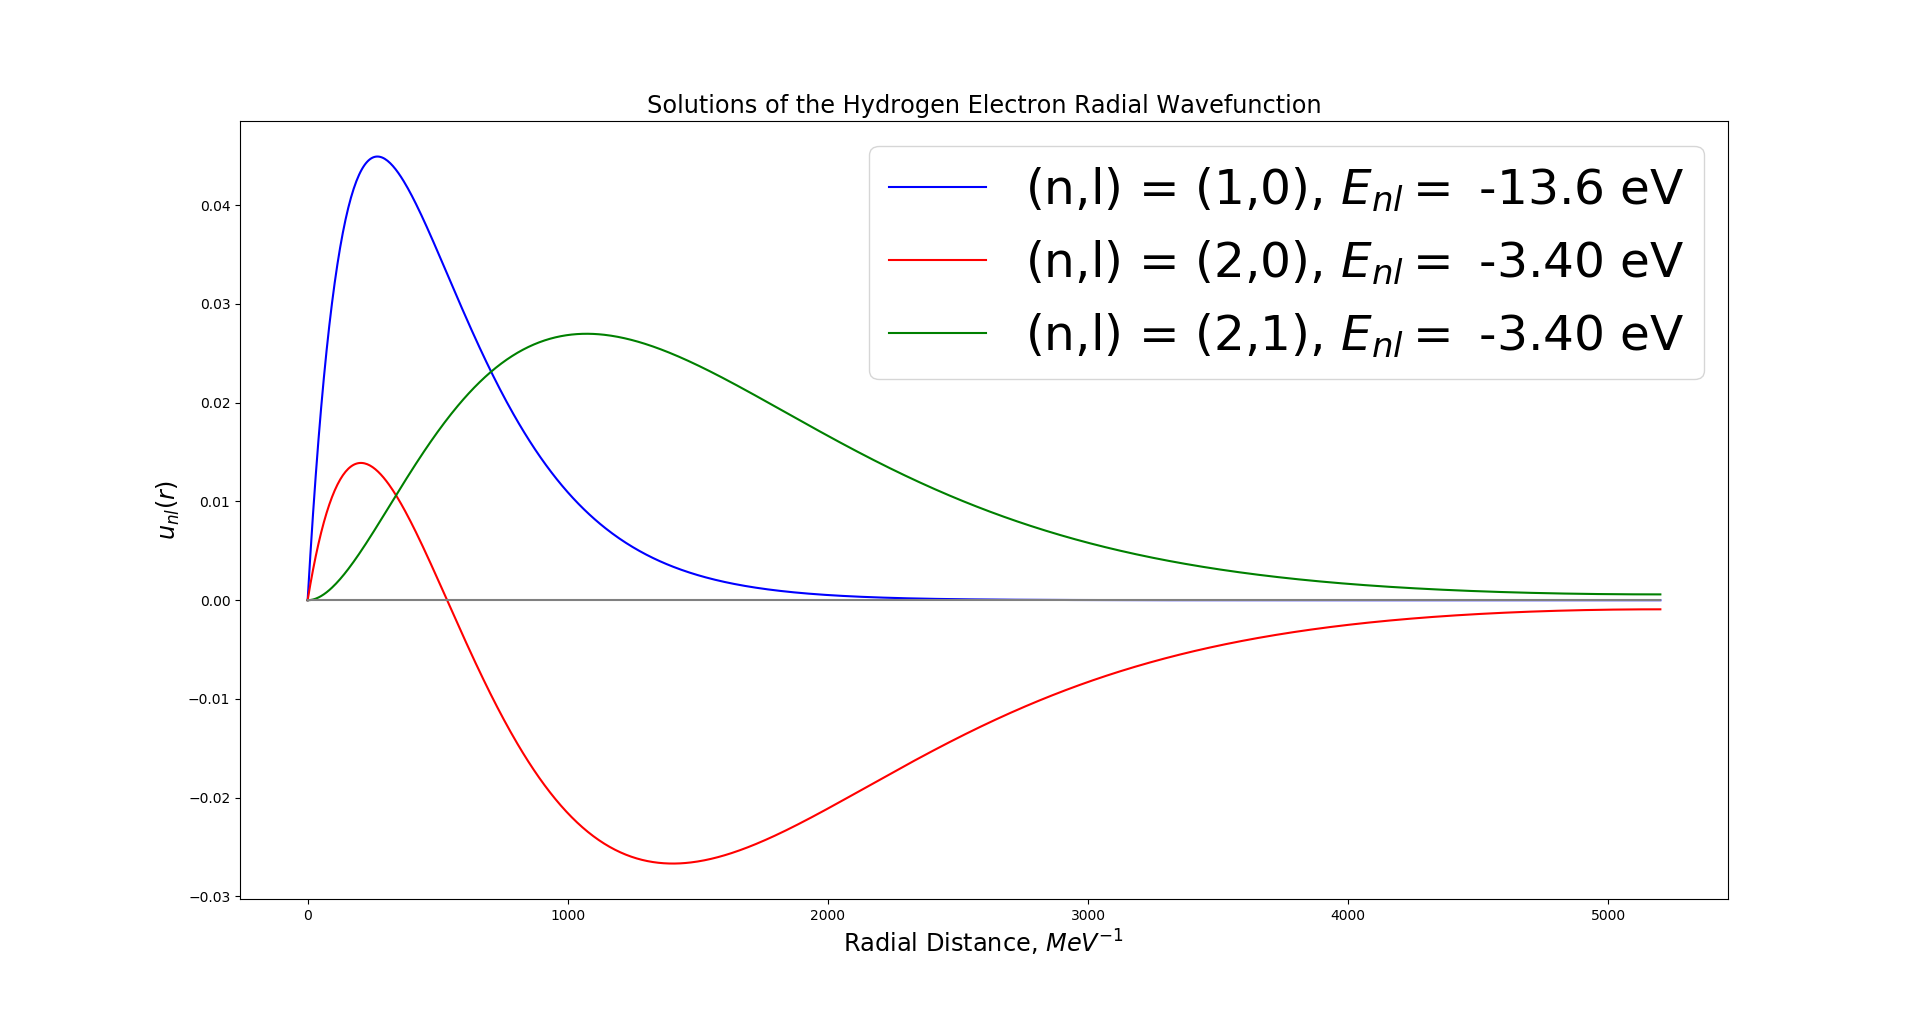
\includegraphics[width=\linewidth]{Hydro}
    \end{figure}
}

\end{poster}%
%
\end{document}
